\documentclass[]{article}
\usepackage{lmodern}
\usepackage{amssymb,amsmath}
\usepackage{ifxetex,ifluatex}
\usepackage{fixltx2e} % provides \textsubscript
\ifnum 0\ifxetex 1\fi\ifluatex 1\fi=0 % if pdftex
  \usepackage[T1]{fontenc}
  \usepackage[utf8]{inputenc}
\else % if luatex or xelatex
  \ifxetex
    \usepackage{mathspec}
    \usepackage{xltxtra,xunicode}
  \else
    \usepackage{fontspec}
  \fi
  \defaultfontfeatures{Mapping=tex-text,Scale=MatchLowercase}
  \newcommand{\euro}{€}
\fi
% use upquote if available, for straight quotes in verbatim environments
\IfFileExists{upquote.sty}{\usepackage{upquote}}{}
% use microtype if available
\IfFileExists{microtype.sty}{%
\usepackage{microtype}
\UseMicrotypeSet[protrusion]{basicmath} % disable protrusion for tt fonts
}{}
\usepackage[margin=1in]{geometry}
\usepackage{color}
\usepackage{fancyvrb}
\newcommand{\VerbBar}{|}
\newcommand{\VERB}{\Verb[commandchars=\\\{\}]}
\DefineVerbatimEnvironment{Highlighting}{Verbatim}{commandchars=\\\{\}}
% Add ',fontsize=\small' for more characters per line
\usepackage{framed}
\definecolor{shadecolor}{RGB}{248,248,248}
\newenvironment{Shaded}{\begin{snugshade}}{\end{snugshade}}
\newcommand{\KeywordTok}[1]{\textcolor[rgb]{0.13,0.29,0.53}{\textbf{{#1}}}}
\newcommand{\DataTypeTok}[1]{\textcolor[rgb]{0.13,0.29,0.53}{{#1}}}
\newcommand{\DecValTok}[1]{\textcolor[rgb]{0.00,0.00,0.81}{{#1}}}
\newcommand{\BaseNTok}[1]{\textcolor[rgb]{0.00,0.00,0.81}{{#1}}}
\newcommand{\FloatTok}[1]{\textcolor[rgb]{0.00,0.00,0.81}{{#1}}}
\newcommand{\CharTok}[1]{\textcolor[rgb]{0.31,0.60,0.02}{{#1}}}
\newcommand{\StringTok}[1]{\textcolor[rgb]{0.31,0.60,0.02}{{#1}}}
\newcommand{\CommentTok}[1]{\textcolor[rgb]{0.56,0.35,0.01}{\textit{{#1}}}}
\newcommand{\OtherTok}[1]{\textcolor[rgb]{0.56,0.35,0.01}{{#1}}}
\newcommand{\AlertTok}[1]{\textcolor[rgb]{0.94,0.16,0.16}{{#1}}}
\newcommand{\FunctionTok}[1]{\textcolor[rgb]{0.00,0.00,0.00}{{#1}}}
\newcommand{\RegionMarkerTok}[1]{{#1}}
\newcommand{\ErrorTok}[1]{\textbf{{#1}}}
\newcommand{\NormalTok}[1]{{#1}}
\usepackage{graphicx}
\makeatletter
\def\maxwidth{\ifdim\Gin@nat@width>\linewidth\linewidth\else\Gin@nat@width\fi}
\def\maxheight{\ifdim\Gin@nat@height>\textheight\textheight\else\Gin@nat@height\fi}
\makeatother
% Scale images if necessary, so that they will not overflow the page
% margins by default, and it is still possible to overwrite the defaults
% using explicit options in \includegraphics[width, height, ...]{}
\setkeys{Gin}{width=\maxwidth,height=\maxheight,keepaspectratio}
\ifxetex
  \usepackage[setpagesize=false, % page size defined by xetex
              unicode=false, % unicode breaks when used with xetex
              xetex]{hyperref}
\else
  \usepackage[unicode=true]{hyperref}
\fi
\hypersetup{breaklinks=true,
            bookmarks=true,
            pdfauthor={Juan Navarro},
            pdftitle={Regression Models Report},
            colorlinks=true,
            citecolor=blue,
            urlcolor=blue,
            linkcolor=magenta,
            pdfborder={0 0 0}}
\urlstyle{same}  % don't use monospace font for urls
\setlength{\parindent}{0pt}
\setlength{\parskip}{6pt plus 2pt minus 1pt}
\setlength{\emergencystretch}{3em}  % prevent overfull lines
\setcounter{secnumdepth}{0}

%%% Use protect on footnotes to avoid problems with footnotes in titles
\let\rmarkdownfootnote\footnote%
\def\footnote{\protect\rmarkdownfootnote}

%%% Change title format to be more compact
\usepackage{titling}
\setlength{\droptitle}{-2em}
  \title{Regression Models Report}
  \pretitle{\vspace{\droptitle}\centering\huge}
  \posttitle{\par}
  \author{Juan Navarro}
  \preauthor{\centering\large\emph}
  \postauthor{\par}
  \predate{\centering\large\emph}
  \postdate{\par}
  \date{Sunday, March 22, 2015}




\begin{document}

\maketitle


\section{Miles per Gallon and How Tranmission Affects
It}\label{miles-per-gallon-and-how-tranmission-affects-it}

\section{Executive Summary}\label{executive-summary}

This is a report for the Regression Models assignment project of the
Coursera Data Science Specialization. It is required in this project to
analyze the mtcars dataset provided by R and explore the relationship
between its variables and the mpg variable (miles per gallon) of the
cars.

The goal is to be able to answer the following questions:

Is an automatic or manual transmission better for MPG?

Can we quantify how different the MPG is between the transmission types?

The main results of this analysis are that: A better value of the miles
per gallon variable (mpg) are found with manual transmissions. There is
an aproximated increase of 1.8 MPG when switching from an automatic
transmission to a manual one.

\section{Data Processing}\label{data-processing}

We begin by loading in the mtcars dataset and transforming certain
variables into factors.

\begin{Shaded}
\begin{Highlighting}[]
\KeywordTok{data}\NormalTok{(mtcars)}
\NormalTok{mtcars$am <-}\StringTok{ }\KeywordTok{factor}\NormalTok{(mtcars$am,}\DataTypeTok{labels=}\KeywordTok{c}\NormalTok{(}\StringTok{"Automatic"}\NormalTok{,}\StringTok{"Manual"}\NormalTok{))}
\NormalTok{mtcars$gear <-}\StringTok{ }\KeywordTok{factor}\NormalTok{(mtcars$gear)}
\NormalTok{mtcars$cyl <-}\StringTok{ }\KeywordTok{factor}\NormalTok{(mtcars$cyl)}
\NormalTok{mtcars$vs <-}\StringTok{ }\KeywordTok{factor}\NormalTok{(mtcars$vs)}
\NormalTok{mtcars$carb <-}\StringTok{ }\KeywordTok{factor}\NormalTok{(mtcars$carb)}
\end{Highlighting}
\end{Shaded}

\section{\#\#Exploratory Analysis}\label{exploratory-analysis}

At first, in order to understand the data, I simply took a look at the
relationships between the many variables present in the dataset. Making
a set of scatterplots comparing each pair of variables as in the
following graph.

\begin{Shaded}
\begin{Highlighting}[]
\KeywordTok{pairs}\NormalTok{(mpg ~}\StringTok{ }\NormalTok{., }\DataTypeTok{data =} \NormalTok{mtcars)}
\end{Highlighting}
\end{Shaded}

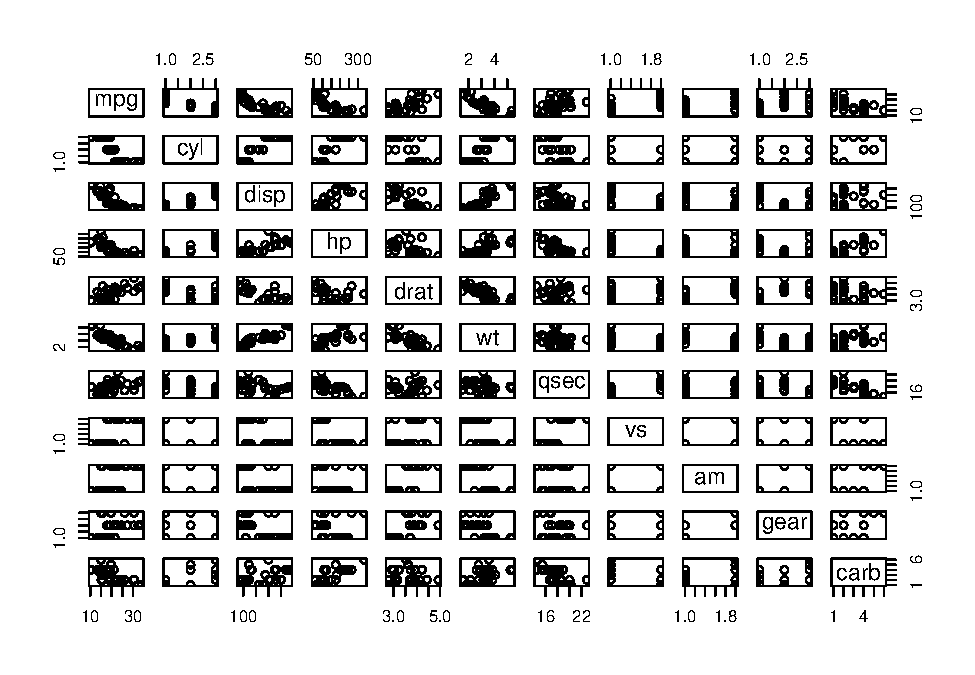
\includegraphics{regression_models_report_files/figure-latex/unnamed-chunk-2-1.pdf}

It is possible to observe that many variables, such as cyl, disp, wt,
hp, drat, vs, am, and carb, have correlations with mpg. Therefore I must
consider this variables for the fitting of the linear model too.

The relationship of interest for this analysis is between the am factor
variable and mpg. I must look at the distribution of mpg for each of the
two levels of am. This can be more easily seen in the following boxplot.
It is clear that manual transmissions tend to have higher MPG.

\begin{Shaded}
\begin{Highlighting}[]
\KeywordTok{boxplot}\NormalTok{(mpg ~}\StringTok{ }\NormalTok{am, }\DataTypeTok{data =} \NormalTok{mtcars, }\DataTypeTok{col =} \NormalTok{(}\KeywordTok{c}\NormalTok{(}\StringTok{"green"}\NormalTok{,}\StringTok{"red"}\NormalTok{)), }\DataTypeTok{ylab =} \StringTok{"Miles Per Gallon (mpg)"}\NormalTok{, }\DataTypeTok{xlab =} \StringTok{"Transmission Type (am)"}\NormalTok{)}
\end{Highlighting}
\end{Shaded}

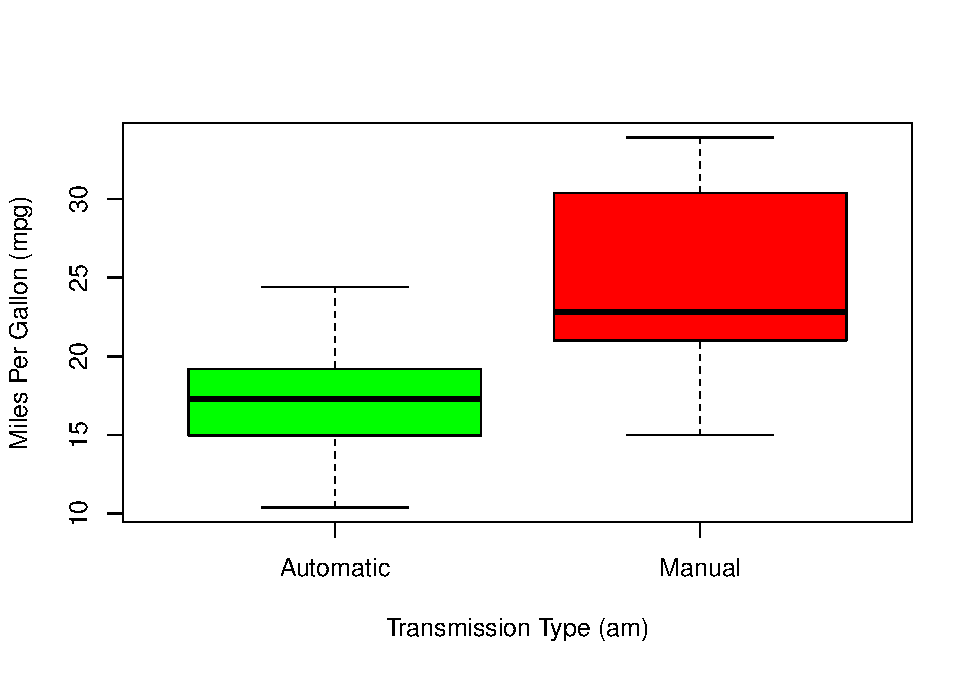
\includegraphics{regression_models_report_files/figure-latex/unnamed-chunk-3-1.pdf}

\section{Regression Analysis}\label{regression-analysis}

In first place, using all the variables to predict mpg I fit a lineal
model and then I will try to choose the most significant predictors for
the definitive model. The step function performs this selection by
calling lm several times. The best variables are selected to be used in
predicting mpg with the Akaike information criterion that implements
both forward selection and backward elimination. By this I can be sure
that I have included the most relevant variables and not included those
unrelated ones that do not contribute significantly to predicting the
variable of interest.

\begin{Shaded}
\begin{Highlighting}[]
\NormalTok{initial_model <-}\StringTok{ }\KeywordTok{lm}\NormalTok{(mpg ~}\StringTok{ }\NormalTok{., }\DataTypeTok{data =} \NormalTok{mtcars)}
\NormalTok{best_model <-}\StringTok{ }\KeywordTok{step}\NormalTok{(initial_model, }\DataTypeTok{direction =} \StringTok{"both"}\NormalTok{)}
\end{Highlighting}
\end{Shaded}

\begin{verbatim}
## Start:  AIC=76.4
## mpg ~ cyl + disp + hp + drat + wt + qsec + vs + am + gear + carb
## 
##        Df Sum of Sq    RSS    AIC
## - carb  5   13.5989 134.00 69.828
## - gear  2    3.9729 124.38 73.442
## - am    1    1.1420 121.55 74.705
## - qsec  1    1.2413 121.64 74.732
## - drat  1    1.8208 122.22 74.884
## - cyl   2   10.9314 131.33 75.184
## - vs    1    3.6299 124.03 75.354
## <none>              120.40 76.403
## - disp  1    9.9672 130.37 76.948
## - wt    1   25.5541 145.96 80.562
## - hp    1   25.6715 146.07 80.588
## 
## Step:  AIC=69.83
## mpg ~ cyl + disp + hp + drat + wt + qsec + vs + am + gear
## 
##        Df Sum of Sq    RSS    AIC
## - gear  2    5.0215 139.02 67.005
## - disp  1    0.9934 135.00 68.064
## - drat  1    1.1854 135.19 68.110
## - vs    1    3.6763 137.68 68.694
## - cyl   2   12.5642 146.57 68.696
## - qsec  1    5.2634 139.26 69.061
## <none>              134.00 69.828
## - am    1   11.9255 145.93 70.556
## - wt    1   19.7963 153.80 72.237
## - hp    1   22.7935 156.79 72.855
## + carb  5   13.5989 120.40 76.403
## 
## Step:  AIC=67
## mpg ~ cyl + disp + hp + drat + wt + qsec + vs + am
## 
##        Df Sum of Sq    RSS    AIC
## - drat  1    0.9672 139.99 65.227
## - cyl   2   10.4247 149.45 65.319
## - disp  1    1.5483 140.57 65.359
## - vs    1    2.1829 141.21 65.503
## - qsec  1    3.6324 142.66 65.830
## <none>              139.02 67.005
## - am    1   16.5665 155.59 68.608
## - hp    1   18.1768 157.20 68.937
## + gear  2    5.0215 134.00 69.828
## - wt    1   31.1896 170.21 71.482
## + carb  5   14.6475 124.38 73.442
## 
## Step:  AIC=65.23
## mpg ~ cyl + disp + hp + wt + qsec + vs + am
## 
##        Df Sum of Sq    RSS    AIC
## - disp  1    1.2474 141.24 63.511
## - vs    1    2.3403 142.33 63.757
## - cyl   2   12.3267 152.32 63.927
## - qsec  1    3.1000 143.09 63.928
## <none>              139.99 65.227
## + drat  1    0.9672 139.02 67.005
## - hp    1   17.7382 157.73 67.044
## - am    1   19.4660 159.46 67.393
## + gear  2    4.8033 135.19 68.110
## - wt    1   30.7151 170.71 69.574
## + carb  5   13.0509 126.94 72.095
## 
## Step:  AIC=63.51
## mpg ~ cyl + hp + wt + qsec + vs + am
## 
##        Df Sum of Sq    RSS    AIC
## - qsec  1     2.442 143.68 62.059
## - vs    1     2.744 143.98 62.126
## - cyl   2    18.580 159.82 63.466
## <none>              141.24 63.511
## + disp  1     1.247 139.99 65.227
## + drat  1     0.666 140.57 65.359
## - hp    1    18.184 159.42 65.386
## - am    1    18.885 160.12 65.527
## + gear  2     4.684 136.55 66.431
## - wt    1    39.645 180.88 69.428
## + carb  5     2.331 138.91 72.978
## 
## Step:  AIC=62.06
## mpg ~ cyl + hp + wt + vs + am
## 
##        Df Sum of Sq    RSS    AIC
## - vs    1     7.346 151.03 61.655
## <none>              143.68 62.059
## - cyl   2    25.284 168.96 63.246
## + qsec  1     2.442 141.24 63.511
## - am    1    16.443 160.12 63.527
## + disp  1     0.589 143.09 63.928
## + drat  1     0.330 143.35 63.986
## + gear  2     3.437 140.24 65.284
## - hp    1    36.344 180.02 67.275
## - wt    1    41.088 184.77 68.108
## + carb  5     3.480 140.20 71.275
## 
## Step:  AIC=61.65
## mpg ~ cyl + hp + wt + am
## 
##        Df Sum of Sq    RSS    AIC
## <none>              151.03 61.655
## - am    1     9.752 160.78 61.657
## + vs    1     7.346 143.68 62.059
## + qsec  1     7.044 143.98 62.126
## - cyl   2    29.265 180.29 63.323
## + disp  1     0.617 150.41 63.524
## + drat  1     0.220 150.81 63.608
## + gear  2     1.361 149.66 65.365
## - hp    1    31.943 182.97 65.794
## - wt    1    46.173 197.20 68.191
## + carb  5     5.633 145.39 70.438
\end{verbatim}

From the best model we see that in addition to am, also the following
variables are strongly related wt, hp, cyl and therefore useful in
predicting mpg.

\begin{Shaded}
\begin{Highlighting}[]
\KeywordTok{summary}\NormalTok{(best_model)}
\end{Highlighting}
\end{Shaded}

\begin{verbatim}
## 
## Call:
## lm(formula = mpg ~ cyl + hp + wt + am, data = mtcars)
## 
## Residuals:
##     Min      1Q  Median      3Q     Max 
## -3.9387 -1.2560 -0.4013  1.1253  5.0513 
## 
## Coefficients:
##             Estimate Std. Error t value Pr(>|t|)    
## (Intercept) 33.70832    2.60489  12.940 7.73e-13 ***
## cyl6        -3.03134    1.40728  -2.154  0.04068 *  
## cyl8        -2.16368    2.28425  -0.947  0.35225    
## hp          -0.03211    0.01369  -2.345  0.02693 *  
## wt          -2.49683    0.88559  -2.819  0.00908 ** 
## amManual     1.80921    1.39630   1.296  0.20646    
## ---
## Signif. codes:  0 '***' 0.001 '**' 0.01 '*' 0.05 '.' 0.1 ' ' 1
## 
## Residual standard error: 2.41 on 26 degrees of freedom
## Multiple R-squared:  0.8659, Adjusted R-squared:  0.8401 
## F-statistic: 33.57 on 5 and 26 DF,  p-value: 1.506e-10
\end{verbatim}

Comparing this best model that includes all the relevant variables and
the initial simple model that uses only am (the transmission type) as a
predictor for mpg, it is possible to observe that the p-value of the
best model is very low, and therefore I can reject the null hypothesis
that these variables do not contribute to the model fit. Anyway, the
p-value for the simple model, is very high (in comparison with the best
model) and therefore I cannot reject the null hypothesis that the
additional variables it includes are not related enough.

\begin{Shaded}
\begin{Highlighting}[]
\NormalTok{simple_model <-}\StringTok{ }\KeywordTok{lm}\NormalTok{(mpg ~}\StringTok{ }\NormalTok{am, }\DataTypeTok{data =} \NormalTok{mtcars)}
\KeywordTok{anova}\NormalTok{(simple_model,best_model,initial_model)}
\end{Highlighting}
\end{Shaded}

\begin{verbatim}
## Analysis of Variance Table
## 
## Model 1: mpg ~ am
## Model 2: mpg ~ cyl + hp + wt + am
## Model 3: mpg ~ cyl + disp + hp + drat + wt + qsec + vs + am + gear + carb
##   Res.Df    RSS Df Sum of Sq       F    Pr(>F)    
## 1     30 720.90                                   
## 2     26 151.03  4    569.87 17.7489 1.476e-05 ***
## 3     15 120.40 11     30.62  0.3468    0.9588    
## ---
## Signif. codes:  0 '***' 0.001 '**' 0.01 '*' 0.05 '.' 0.1 ' ' 1
\end{verbatim}

\section{Model Evaluation}\label{model-evaluation}

Analyzing the Residuals vs Fitted plot it is possible to observe that
the residuals are randomly scattered and verifying this way, the
independece condition. If there is any pattern would present, it would
indicate underfitting of the model. In Normal Q-Q plot it is possible to
read that the residuals are approximately normally distributed.

The data points with the most leverage in the fit can be found by
looking at the hatvalues(). Those that influence the model coefficients
the most are given by the dfbetas() function.

\begin{Shaded}
\begin{Highlighting}[]
\KeywordTok{par}\NormalTok{(}\DataTypeTok{mfrow=}\KeywordTok{c}\NormalTok{(}\DecValTok{2}\NormalTok{, }\DecValTok{2}\NormalTok{))}
\KeywordTok{plot}\NormalTok{(best_model)}
\end{Highlighting}
\end{Shaded}

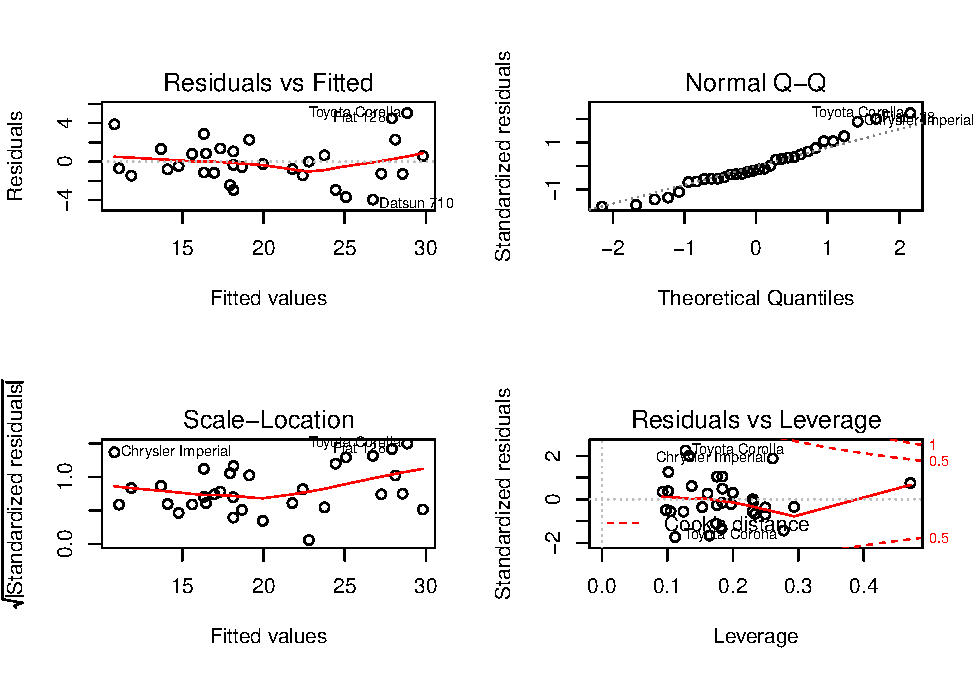
\includegraphics{regression_models_report_files/figure-latex/unnamed-chunk-7-1.pdf}

\section{Statstical Inference}\label{statstical-inference}

Finally I performed a t-test on the two subsets of mpg data: manual and
automatic transmissions. It is assumed for this test that both are
normally distributed and tests the null hypothesis that they come from
the same distribution. This performs a two-sided test with α=0.05 and
assuming unequal variances. The t-test results as shown allow us to
reject the null hypothesis that the mpg distributions for manual and
automatic transmissions are the same.

\begin{Shaded}
\begin{Highlighting}[]
\KeywordTok{t.test}\NormalTok{(mpg ~}\StringTok{ }\NormalTok{am, }\DataTypeTok{data =} \NormalTok{mtcars)}
\end{Highlighting}
\end{Shaded}

\begin{verbatim}
## 
##  Welch Two Sample t-test
## 
## data:  mpg by am
## t = -3.7671, df = 18.332, p-value = 0.001374
## alternative hypothesis: true difference in means is not equal to 0
## 95 percent confidence interval:
##  -11.280194  -3.209684
## sample estimates:
## mean in group Automatic    mean in group Manual 
##                17.14737                24.39231
\end{verbatim}

\section{Conclusions}\label{conclusions}

After perfoming several model fits to find the best model I showed that
the selected model was better than a simple model (using only am to
predict mpg) and at the same time it does not include unnecessary
variables in the fit. The folling can be concluded:

There is a decrease of aproximately 0.32 in MPG for every increase of 10
in horsepower.

MPG also decreases near 2.5 for every 1000 lb increase in the weight of
the vehicle.

MPG will decrease by 3.0 or 2.2 When the number of cylinders increases
from 4 to 6 or 8 respectively.

Manual transmissions get 1.8 more MPG than automatic cars. This is
considering also horsepower, the weight and the number of cylinders of
the car

\end{document}
